\documentclass{emulateapj}
%\documentclass[12pt,preprint]{aastex}

\usepackage{graphicx}
\usepackage{float}
\usepackage{amsmath}
\usepackage{epsfig,floatflt}
\usepackage{hyperref}
\usepackage[utf8]{inputenc}
\usepackage{listings}
\usepackage{color}
\usepackage{url}


\lstset{language=c++}
\lstset{alsolanguage=[90]Fortran}
\lstset{alsolanguage=Python}
\lstset{basicstyle=\small}
\lstset{backgroundcolor=\color{white}}
\lstset{frame=single}
\lstset{stringstyle=\ttfamily}
\lstset{keywordstyle=\color{red}\bfseries}
\lstset{commentstyle=\itshape\color{blue}}
\lstset{showspaces=false}
\lstset{showstringspaces=false}
\lstset{showtabs=false}
\lstset{breaklines}



\begin{document}

\title{Colors on a CCD; cleaning an image and using a diffraction pattern to find the pixel size.}

\author{Daniel Heinesen}

\email{daniel.heinesen@sf-nett.no}

\altaffiltext{1}{Institute of Theoretical Astrophysics, University of
  Oslo, P.O.\ Box 1029 Blindern, N-0315 Oslo, Norway}


%\date{Received - / Accepted -}

\begin{abstract}
  In this article we are looking at the new imaging tool charge coupled device. First we looked at how white light was separated to it constituent colors when passing through a lens, and how the CCD captured this. This was done by sending white light through a thin lens and an objective. We saw how due to aberrations in the lens we got different colors focusing at different distances from the lens. Even though the focused light look at a first glans to be monochromatic, most of the colors are present in some amount. We then pointed a laser on a single slit, making a diffraction pattern on the CCD. We could use this diffraction pattern to find a pixel size of $(5.45 \pm 0.32)\text{ }\mu\text{m}$. We also looked at the different noises made by imperfections in the instruments: the bias, dark current and flat field. We used multiple flat frames taken with uniform light to see that the more flat frames the more the noise decreased. An ideal decrease would have been on the order $1/\sqrt{n}$, but out data showed closer to $1/n$. Lastly we cleaned an image of the diffraction pattern with the use of flat frames and dark frames. The corrected image showed little to no difference, which may have been to the flaw in setting up the flat frame.
\end{abstract}
\keywords{Charge-coupled devise --- CCD --- Pixel Size --- Single Slit --- Lens --- Image cleaning --- Flat field --- Dark Frame --- Bias}

\section{Introduction}
\label{sec:introduction}

In this article we are going to look at some properties of the charge-coupled device, CCD. This is a new method of capturing light using CMOS semiconductors to convert photons in to an electric current. The CCD had $50-90\%$ efficiency, compared to the $\sim 1\%$ efficiency for normal photographic plates. This means that CCDs may revolutionize the way we observe the universe. \\

CCD-chips are able to capturing red, green and blue light, and therefore able to replicate any colors the observed object may have. A white light shined through a thin lens will make a diffraction patter, and an Airy disk. The lens will also separate the white light into its constitute colors, due to chromatic aberrations. We are going to look at the different focal points of these colors. The light captured may look monochromatic, but as we shall see, red, green and blue are always there, in some amount or another. \\

We are then going to change the color camera with a monochromatic camera, and the lens with a slit. This will make diffraction pattern on the CCD. With the use of this diffraction pattern it is possible to find the size of the pixels.\\

Due to imperfections in the CCD and other instruments there will be noise in the images: the bias(noise in the electronics), dark current(current due to thermal effects) and flat field(imperfections in the pixels and in the other instruments) . We will especially look at the noise made by the bias  and flat field , and how we can decrease this noise be using many flat frames. \\

By isolating images of the bias, dark current and flat field, it is possible to correct for these imperfections and get a clearer image. We will use this to clean the image of the diffraction pattern.



\section{Theory}
\label{sec:theory}

\subsection{Some Aberrations}

Aberrations are effect due to the lens and bending of light, that leads to curtain unwanted errors in an image.

\subsubsection{Coma}
\label{sec:coma}
Coma is an aberration that happens when the light hits the lens at an angle, leading some of the light to be bend more then other. This effect leads to a comet like picture.

\subsubsection{Chromatic Aberration}
\label{sec:chromAb}
Chromatic aberration happens because the reflective index is dependent on the wavelength of the light. This gives the different colors different focal points.


\subsection{The CCD}
\label{sec:ccd}
This is a short qualitative summary of the inner workings of the charge-coupled device (CCD):

A pixel of the CCD consists of three layers: a doped semiconductor layer (usually some silica), separated from a conducting material by some isolator. 

\begin{figure}[H]
\centering
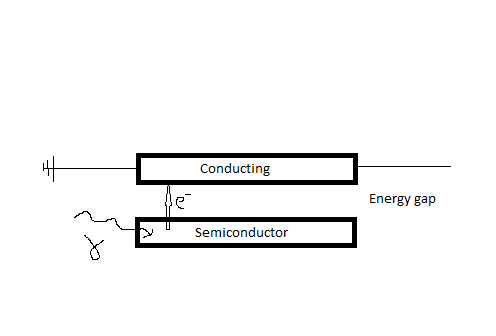
\includegraphics[scale=0.4]{ccd.png}
\caption{A (very) simple illustration of a CCD-chip}
\end{figure}


The isolating layer is characterized by some energy $E_g$ (g for gap). This gap energy is so that electrons from the semiconducting layer cant overcome it and transverse to the conduction layer. But should a photon hit an electron with higher energy then $E_g$, the electron can overcome the gap energy and reach the conduction layer. The wavelength needed to give the electron this energy is called the cut-off wavelength

\begin{equation}
\lambda_{c} = \frac{hc}{E_g}
\end{equation}

Where $h$ is Planck's constant and $c$ the speed of light. This wavelength determines the largest wavelength the CCD is able to detect. 

After the electrons reach the conduction they are lead to a register, who counts the number of electrons. The number of electrons should be proportional to the number of photons hitting the pixel, and from this the number of photons hitting the pixel can be calculated.


\subsection{Finding the Pixel Size}
\label{sec:pixSize}
To find the pixel size we used a slit to make a diffraction pattern on the screen. We can so use the single-slit diffraction pattern

\begin{equation}
a \sin(\theta) = m\lambda
\label{eq:diffPatt}
\end{equation}

Where $a$ is the width of the slit, $m$ is the order of the minimum, $\theta$ is the angle to said minimum and $\lambda$ is the wavelength of the incoming light/laser.

\begin{figure}[H]
\centering
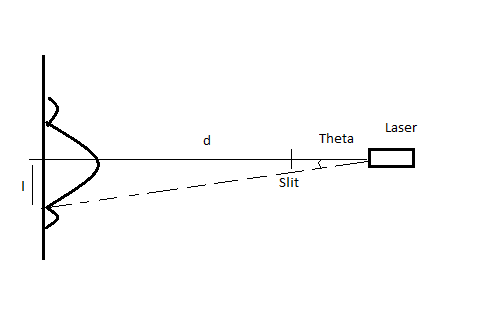
\includegraphics[scale=0.4]{diffPattern.png}
\caption{A crude illustration of the laser and slit. $l$ is the distance to the first minimum and $d$ the the distance from the slit to the CCD}
\end{figure}


If we look at the drawing, we see that the able $\theta$ is given as

\begin{equation}
\tan \theta = \frac{l}{d}
\end{equation}

Where $l$ is the distance to first minimum. But this angle is small, so we can use the small angle approximation $\tan \theta \approx \theta$. The distance $l$ is also not completely known. We know the number of pixels from the center to the first minimum \ref{sec:setup}, but we do not know how this relate to the actual distance. So we say that

\begin{equation}
l = n_{pixels}\cdot c
\end{equation}

Where $n_{pixels}$ is the number of pixels, and $c$ is some conversion factor, given in meters (the number of pixels are dimensionless). Using this and the small angle approximation we get that

\begin{equation}
\theta \approx \frac{n_{pixels}\cdot c}{d}
\end{equation}

We are also going to use the small angle approximation on \eqref{eq:diffPatt} and use our expression for $\theta$

\begin{equation}
m\lambda \approx a\theta = a\frac{n_{pixels}\cdot c}{d}
\end{equation}

This gives us a nice expression for the size of the pixels

\begin{equation}
c \approx \frac{m\lambda d}{n_{pixels}a}
\label{eq:pixelSize}
\end{equation}


$n_{pixels}$ will be found be plotting a slice of the middle of an image of the a diffraction patter. The value for $n_{pixels}$ can then be read from the plot.

\subsection{Different Cleaning Frame}

The three types of 'cleaning images'\footnote{for a lack of a better name}:

\subsubsection{Bias}
When using a CCD there are a lot of electronics involved. The signal travels though a lot of cables. These cables may have either loss or gain of electrons. This normally leads to a constant gain or loss of signal. One of the most important gain in signal is from the electronics needed to take the electrons from the conduction layer of the CCD \ref{sec:ccd} to the register. This needs a constant potential to drive the electrons, which gives a gain in signal.

The bias is additive, meaning that to remove it we need to quantify  the bias, then subtract it from the scientific image. To quantify the bias we take pictures without any light hitting the CCD, capturing only the signal from the electronics.\footnote{We will also capture the dark current, but for simplicity this is ignored.}

\subsubsection{Dark Current}
As mentioned in sec. \ref{sec:ccd} the barrier between the semiconductor and conducting layer is given as an energy $E_g$. Ideally this energy gap is so large that no electron will wander across it unless exited by a photon. But this is a quantum system it is never that easy. The energy of the electron follows a Fermi-Dirac distribution \citep{wiki:fermi}

\begin{equation}
P(E,T) = \frac{1}{1 + e^{(E-E_f)/kT}}
\end{equation}

Where $E$ is the energy of the electron, $T$ the temperature, $E_f$ the Fermi energy and $k$ the Boltzmann's constant. Thus for larger temperatures we are more likely to find electrons with a high energy. Meaning that for normal room temperature, there will be electrons that, due to quantum mechanics, will have enough energy to overcome the energy gap and reach the conducting layer. So even though there are no light, the CCD may register signals. This is dark current.

Just like the bias, dark current is additive, and must be subtracted from the raw scientific image. The value of the dark current is found be taking pictures without light.

\subsubsection{Flat Field}
Maybe the most important correction image is the flat field. Flat fields may be the result of many things. Due to differing efficiency from pixel to pixel in the CCD, the signal may not be uniform over the whole picture, even though the same light is shined upon all the pixels. 

There may also be dust on the lenses or other imperfections. This is also adjusted with the flat field.

The flat field is multiplicative, and is adjusted for by dividing the raw scientific image by the flat frames. Since the flat field is due to imperfections in the pixels and on the lenses(and other instrument before the CCD), we want to take an image of a uniformly lit image. This gives us the flat frame.\footnote{I may use flat field and flat frame interchangeably throughout the text, but they are taken to mean the same: the image of the uniform lit background.}

\subsection{Statistical Analysis}
To clean the images we want ideal flat field, dark frames and bias frames. But this is not the case. There are some noise in the images. This is characterized as the deviation from the mean of the image, or the standard deviation $\sigma$.

\subsubsection{Noise of the Bias}
\label{sec:noiseBias}
For the bias frames we wan to look at just the noise which is not constant. We therefore subtract the two bias frames $B_1 - B_2$. This removes all the constant noise, leaving us with only the undesired variable noise. We can then find the standard deviation of this $\sigma_{B_1 - B_2}$. If we look at the addition rules of variance \citep{wiki:var} we see

\begin{equation}
Var(aX - bY) = a^2Var(X) + b^2Var(b)
\end{equation}

We then get:

\begin{equation}
\sigma_{B_1 - B_2}^2 = \sigma_{B_1}^2 + \sigma_{B_2}^2
\end{equation}

We expect that the noise in the bias frames should be constant over time, so the standard deviation, and thus variance, for the two bias frames should be equal\footnote{Breaking the fourth wall: I'm not sure about this line of reason, but it gives the correct answer, so I included it.}. So

\begin{equation}
\sigma_{B_1 - B_2}^2 = 2\sigma_{B}^2 \Rightarrow \sigma_{B_1 - B_2} = \sqrt{2}\sigma_B
\label{eq:stdB1B2}
\end{equation}

Then thus we see that the standard deviation of the difference of the biases are $\sqrt{2}$ times that of a single bias frame.

We can also look at the mean of the sum of the two bias frames. Since the mean is linear we get that

\begin{equation}
E(B_1 + B_2) = E(B_1) + E(B_2)
\label{eq:meanB}
\end{equation}

\subsubsection{Noise of the Flat Frames}
\label{sec:noiseFlat}
The same is done with the flat frames. But we want to decrease noise of the flat field, and not increase it as it did in \eqref{eq:stdB1B2}. For that we use several flat fields. So we want to calculate

\begin{equation}
\sigma_{(F_1 + \ldots F_{2n})- (F_2 + \ldots F_{2n+1})}
\end{equation}

Using $n$ pairs of flat fields. But since we have added several frames, the scale of the noise increase with $n$. So we need to normalize with $n$. So what we want to calculate is

\begin{equation}
\frac{\sigma_{(F_1 + \ldots F_{2n})- (F_2 + \ldots F_{2n+1})}}{n}
\end{equation}

If we now use the same relationship as in \eqref{eq:stdB1B2} we see what we want

\begin{equation}
\frac{\sigma_{(F_1 + \ldots F_{2n})- (F_2 + \ldots F_{2n+1})}}{n} = \frac{\sqrt{n}\sigma_F}{n} = \frac{\sigma_F}{\sqrt{n}}
\end{equation}

So we see that as we include more flat frames, the random noise decreases as $1/\sqrt{n}$, and we are left with a more clean flat frame, which can be used to clean our science image. One would at first think that the noise would increase as $\sqrt{n}$ for each flat frame added, but due the normalization, the noise decrease instead.

\subsubsection{Read Out Noise}

We have now found the noise as the standard deviation of the pixel counts in the flat frame. This is in so called analog-to-digital units (ADU). We want to find the readout noise in electrons, so we need a conversion factor. This is given as

\begin{equation}
g = \frac{F_{electrons}}{\sigma_{electrons}} = \frac{(\bar{F}_1 - \bar{F}_2) + (\bar{B}_1-\bar{B}_2)}{\sigma_{F_1 - F_2}^2 - \sigma_{B_1 - B_2}^2}
\label{eq:g}
\end{equation}

Where $F_i$ is a flat frame and $B_i$ is the corresponding bias frame. The second expression comes from the fact that we use the bias frames to clean the flat frames before finding $g$. This conversion factor measures how many electrons which are needed to generate the signal. We can now find the readout noise as

\begin{equation}
\text{R.O.N} = g\cdot\sigma_{bias}
\end{equation}

Which bias frame is used for this should ideally be the same, since we expect time-independent, constant bias noise.

\subsubsection{Cleaning the Image}
\label{sec:cleaning}
To clean the image we want to remove the effects made be the dark current and flat frame. As mentioned the dark current is additive while the flat field is multiplicative. To remove the noise from the the dark and flat frames, we take the average of multiple frames. But the flat frames do also have dark current, so we need to subtract the the corresponding average dark frame from the average flat frame and normalize it. This is the normalized flat frame. We can then simply clean the raw scientific image of the diffraction pattern by first subtract the average dark frame $D_{I,raw,average}$ and divide by the normalized master flat frame $F_{norm. master}$

\begin{equation}
I_{corrected} = \frac{I_{raw} - D_{I,raw,average}}{F_{norm. master}}
\label{eq:ICorr}
\end{equation}

Where $I_{corrected}$ is the cleaned image of the diffraction pattern.
\section{Method}
\label{sec:method}

\subsection{Color Camera, White Light and Lens}

\begin{figure}[H]
\centering
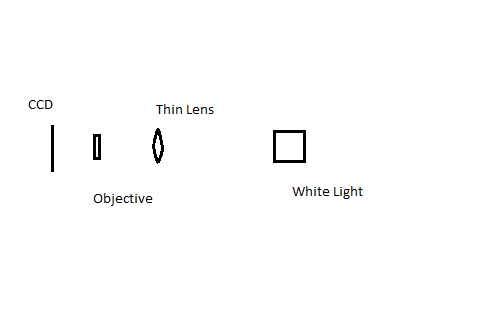
\includegraphics[scale=0.4]{setupLight.png}
\caption{A crude illustration of the setup for the white light.}
\end{figure}

For this first experiment a white light was shined on and focus by a thin single lens. In the focal point of the lens a microscope objective was placed. The focal point of the lens was fond by holding a piece white paper in front of the lens and finding the distance where the light is most concentrated. 

The CCD was then placed in front of the objective. Here we wanted to look at the properties of the different colors in the white light, so a RGB CCD was used\footnote{For this a Edmund Optics color USB camera was used.}. 

We could now use out Graphical User Interface(GUI) to look at the resulting pattern. The result can be described as a histogram showing the amount of light received be the three sensors in the CCD \ref{sec:ccd}. Due to chromatic aberration \ref{sec:chromAb} the different colors focus at different focal length, so to look at this effect we moved the CCD carefully back- and forwards to focus the different colors; red, green and blue.

The GUI gave the possibility of viewing the pixel count of a slice of the image, for the different colors. These values were not saved, but the image itself was. The images was then used to make a plot showing the mean pixel count of each color over each column.

The GUI of the CCD also allowed us to adjust the pixel clock, frame rate and exposure time, giving us the ability to study the effect this had on the picture.

Filters to filter out some of the colors in the white light was placed in front of the light, so we could look on the effect this would have on the light on the CCD. 


\subsection{Monochromatic Camera and Single Slit}

\subsubsection{Setup}
\label{sec:setup}

\begin{figure}[H]
\centering
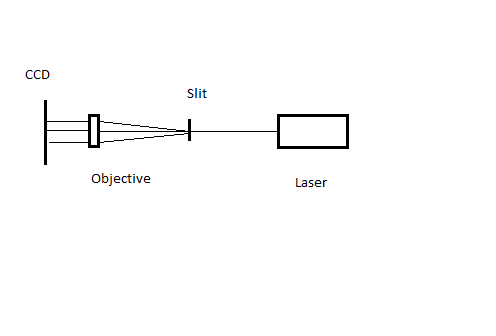
\includegraphics[scale=0.4]{setupLaser.png}
\caption{A crude illustration of the setup for the laser.}
\end{figure}

The white light was now switched out with a monochromatic red laser with wavelength $\lambda = (641 \pm 12.3)$ nm \cite{laser}. To ensure that the laser didn't destroy the CCD, a damping filter was placed in front laser. Then a single slit with a width if $a = 100\mu m$ is placed in front of the laser the laser. The diffracted laser light was then captured by a monochromatic CCD\footnote{A monochromatic Edmund Optics USB camera}. 

The camera and slit was then adjusted until a sharp diffraction pattern appeared in the middle of the computer screen. The distance from the slit to the CCD was so measured carefully with a ruler. Two images image of the diffraction pattern were then taken. One with lower exposer used to calculate the pixel size, described here \ref{sec:pixSize}. The other one, with higher exposer, was used to test out the cleaning procedure \ref{sec:cleaning}.


To clean the picture the following series of pictures were taken \ref{sec:cleaning}. All of the apparatuses were removed, and for all of the pictures except the flat frames (see below) the dust cover was placed on the camera: \\


\begin{itemize}
\item $2$ bias frames with minimum exposer
\item $5$ dark frames with the same exposer as the diffraction pattern
\item $1$ dark frame with maximum exposer
\item $16$ flat frames -- see method below -- with exposer set so that the average pixel value is about half that of max.
\item $5$ dark frames with the same exposer as for the flat frames
\end{itemize}

The flat frames are takes as follows: The dust cover was removed, then a white piece of paper was placed in front of the CCD and a white light was shined on the paper. The white paper ensured a homogeneous, white gradient over the whole CCD chip. With these axillary pictures we could clean the picture of the diffraction pattern.

\subsubsection{Statistical Analysis}
This part was done in Python\ref{sec:code}, but could be found with most other scripting languages, like R or IDL:

First a bias frame and the maximum exposer dark frames has converted to an array. From these arrays the max, min, mean and distribution of the pixel values was found and compared. \\

To find the readout noise we first looked at the two bias frames. To exclude the possibility of strange results near the edge of the picture, a symmetric $300$x$300$ central part was extracted out of the to images and used. The two  images(the central parts) were then added, and the mean pixel value was found. This is the same value as $\bar{B}_1 + \bar{B}_2$\eqref{eq:meanB}. We then calculated the noise for the biases. This was done by first subtracting the images \ref{sec:noiseBias}, then finding the standard deviation of the resulting image $\sigma_{B_1 - B_2}$\eqref{eq:stdB1B2}.

The same was then done for two flat frames -- 2 and 4 -- : first the central regions of the images were found. A mean of the sum of the images was found $\bar{F}_1 + \bar{F}_2$, and then the noise of the difference of the images was found $\sigma_{F_1 - F_2}$.

From this the conversion factor then consequently the readout noise can be calculated \eqref{eq:g}\\

To see how the number of flat frames taken improved the normalized noise, the following was calculated with the same approach as the noise above:
$\sigma_{F_1-F_2}$, $\sigma_{(F_1 + F_3) - (F_2+F_4)}$ and so on until all the flat frames were used. For each time a new $\sigma$ was calculated it was normalized with the number of pairs of flat frames used, then saved. The saved values for the noises were then plotted and compared.\\

To clean the image of the diffraction pattern we generally want to subtract away the noise from the dark frames, and divide away the noise from the flat frames. This was done as follows:

First an average of the $16$ flat frames was found $F_{average}$. An average of the $5$ dark frames corresponding to the flat frame $D_{F,average}$ was then found. We then removed the noise in the average flat frame made by the dark current, giving us the master flat frame $F_{master} = F_{average}-D_{F,average}$. This was then normalized with the scalar mean, giving us $F_{norm. master}$.

Secondly the dark frames corresponding to the image of the diffraction pattern was average to find $D_{I,raw,average}$. 

Finally the final, clean image of the diffraction pattern was given as \eqref{eq:ICorr}:

\begin{equation}
I_{corrected} = \frac{I_{raw} - D_{I,raw,average}}{F_{norm. master}}
\end{equation}

This was done both for the central 300x300 image and the full field of view.



\subsection{Uncertainties}

\subsubsection{Color Camera and White Light and Lens}
\label{sec:uncWhiteLight}
To get a sharp diffraction pattern, the lens, objective and CCD has to be normal to the direction of the path of the light. If the lens is off the normal, we will get a coma, and due to the chromatic aberration in the lens (even thou it is thin, it has a physical thickness) the coma will be enhanced, leading to a smear out of colors(as seen here \ref{img:spekter}). This means that it might be difficult to get a sharp pattern, and the Airy disk might be larger then expected due to this coma, unless the lens is completely normal to the light(fortunately we are not measuring the Airy disk, so this uncertainty is only a curiosity).

When looking at the pixel counts for the different colors, we wanted to look at the pixel count when green dominated. But since green is a mix of blue and yellow, the blue is quite high when ever green is high. So there is quite a small range where green dominates all other colors, including blue. This range was difficult to find by only moving the camera back and forth, so the resulting image does not show very good results.

\subsubsection{Monochromatic Camera and Single Slit}
\label{sec:uncSlit}

Much like with the white light and lens, the quality of the diffraction pattern is dependent on the single slit, objective and CCD being normal to the laser. This was adjusted as best as possible to make this uncertainty as low as possible.
The slit has imperfections in its construction, making the diffraction pattern very uneven, instead of the straight lines we ideally want to see \ref{img:rawPixSize}.
The dominating source of error in our calculations of the pixel size came from the way the number of pixels to the first minimum was found: as one can see in the image of the diffraction pattern \ref{img:rawPixSize} is tilted at an angle, while the plotted slice of the image \ref{img:slice} is take horizontally, meaning that the measured distance to the minimum is larger than the actual distance.
All of these uncertainties has been encompassed by a large, but fair uncertainty of $\pm 5$ pixels. 

The distance from the slit to the camera was measured with a ruler. There was difficulty measuring this distance due to both the exact position of the slit and that of the CCD chip being obscured by their respective casings. So an uncertainty of $\pm 0.2$ cm was added.\\

As will be discussed later \ref{sec:disClean} the way we made the flat field was at best lacking. The bends in the paper, especially at the edges would lead to parts of the paper being darker than the uniform gradient we are looking for. But most grievous error done was taking the flat field without any slit or objective, as will be discussed later.




 
\section{Results}
\label{sec:results}

\subsection{Exposer Times}
\begin{table}[H]
\centering
\begin{tabular}{c|c|c|c}
 & Pixel Clock [Hz] & Frame Rate [fps] & Exposer [ms]\\
 \hline
Color Camera & 7 & 5.32 & 57.309\\
Bias & 5 & 0.18 & 0.08\\
Diffraction Pattern 1 & 40 & 20.61 & 0.08 \\ 
Diffraction Pattern 2 & 40 & 20.61 & 0.124 \\
Flat frames & 5 & 2.58 & 36.883
\end{tabular}
\end{table}


\subsection{Color Camera, White Light and Lens}
\label{sec:resColor}
Image of the full spectrum:

\begin{figure}[H]
\centering
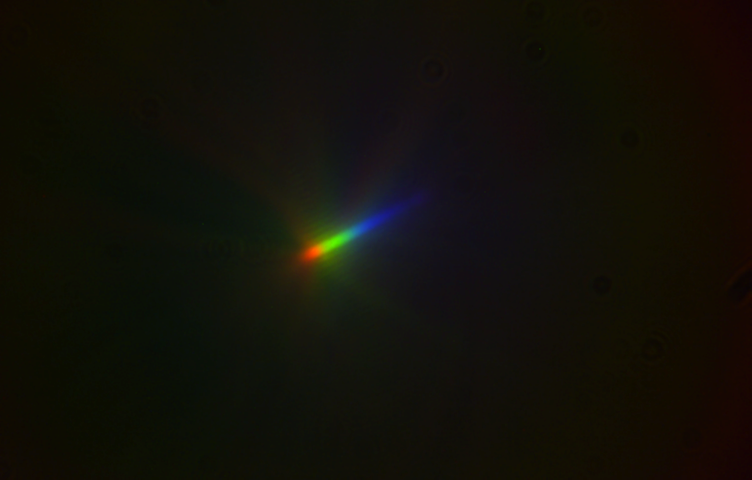
\includegraphics[scale=0.2]{spekter.png}
\caption{Image of the full spectrum. We can see that the comet like spread of the coma, combined with the separation of the different colors due to the chromatic aberration.}
\label{img:spekter}
\end{figure}

Capturing the images for the different colors gave:

\begin{figure}[H]
\centering
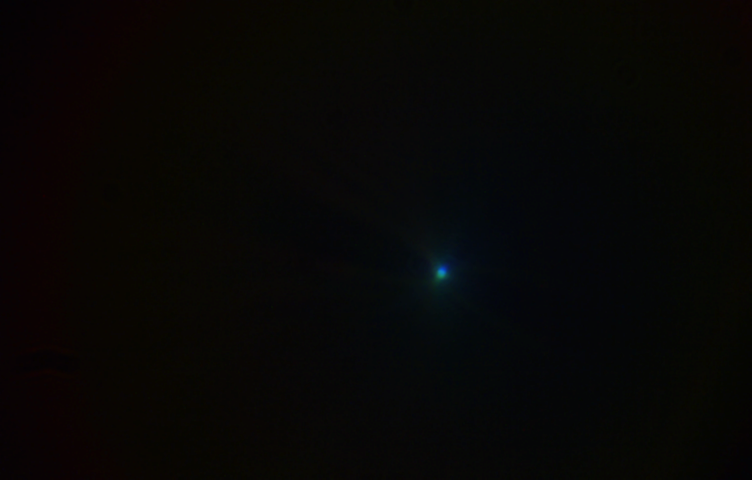
\includegraphics[scale=0.2]{blatt.png}
\caption{Image of blue light in focus.}
\label{img:blue}
\end{figure}
\begin{figure}[H]
\centering
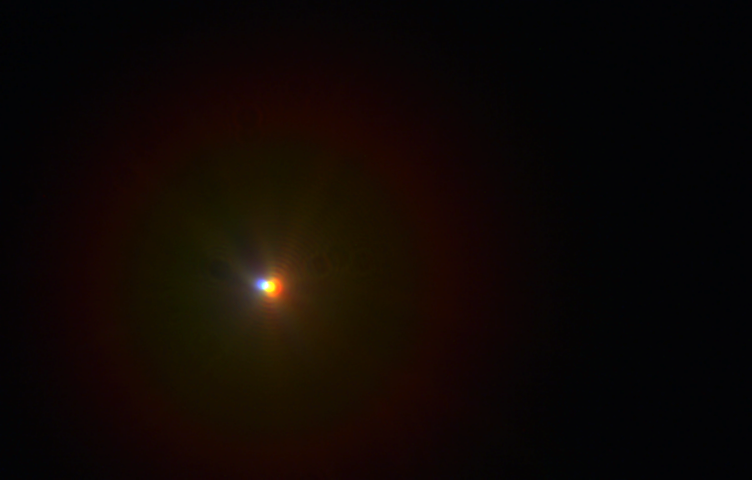
\includegraphics[scale=0.2]{rod_fokus.png}
\caption{Image of red light in focus.}
\label{img:red}
\end{figure}

\begin{figure}[H]
\centering
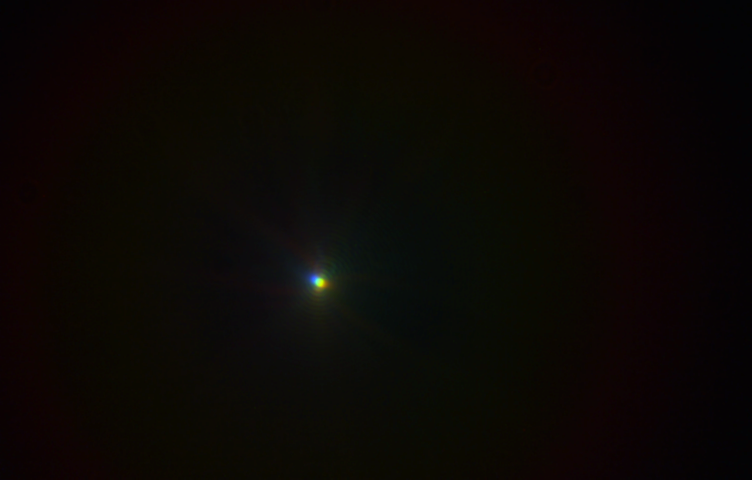
\includegraphics[scale=0.2]{gront_fokus.png}
\caption{Image of green light in focus.}
\label{img:green}
\end{figure}

We can see that for the blue focus it is easy to see that blue dominates. For red it is some what less clear, but we see that there are mostly red light there. But for green the dot in the middle almost looks white, while the ring around looks more red. If we look at the same image but with a red filter we see:

\begin{figure}[H]
\centering
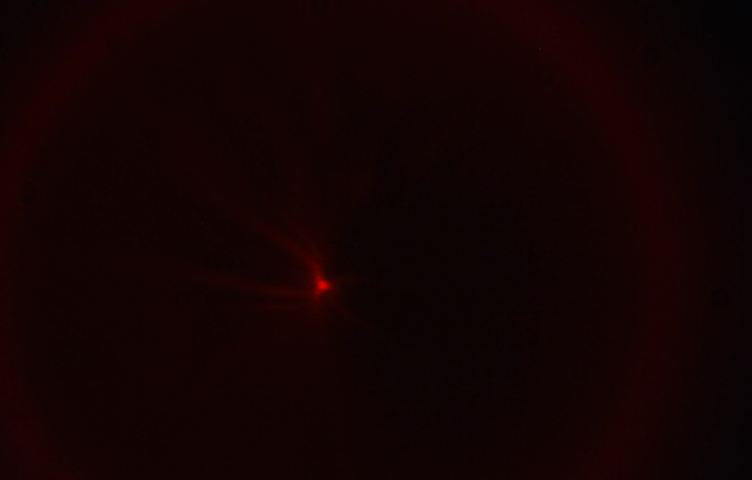
\includegraphics[scale=0.2]{red_filter_green_focus.png}
\caption{Image of green light but with a red filter. As we can see even though we had the CCD in the focal point of the green light, there is a lot of red light too. The reason is mentioned here \ref{sec:uncWhiteLight}}
\label{img:red_filter_green_focus}
\end{figure}

And as we expected there are alot of red in the light light imaged.

These images gave the following distribution:

\begin{figure}[H]
\centering
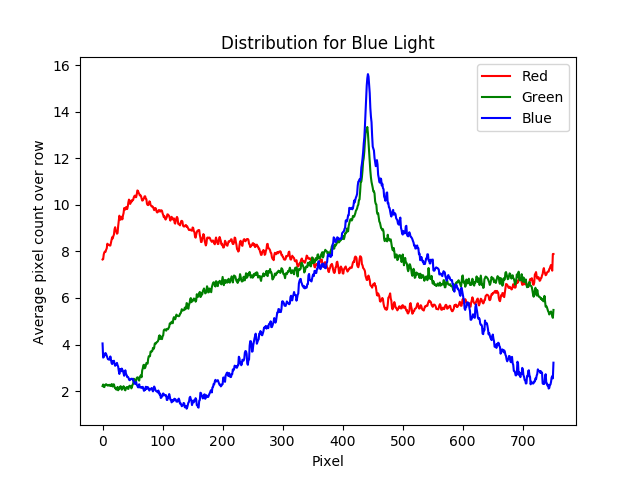
\includegraphics[scale=0.3]{blueDist.png}
\caption{The distribution of the average pixel count for the different colors when in the focal point of the blue light. We can see that blue is dominating, but there are still quite a lot of green light.}
\label{img:blueDist}
\end{figure}

\begin{figure}[H]
\centering
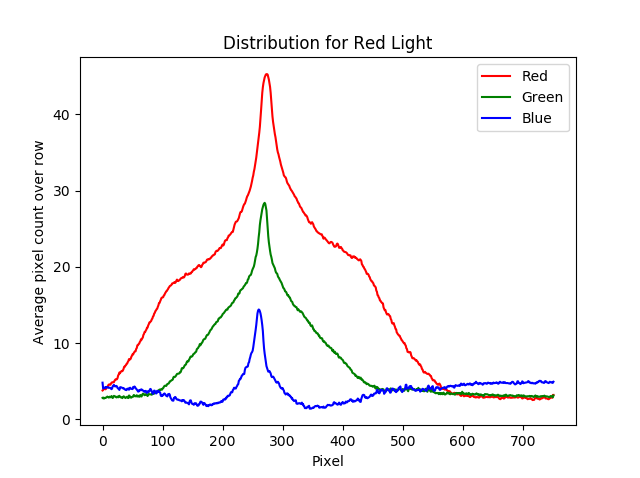
\includegraphics[scale=0.3]{redDist.png}
\caption{The distribution of the average pixel count for the different colors when in the focal point of the red light. We see that red is dominating, while blue is almost non-existent}
\label{img:redDist}
\end{figure}

\begin{figure}[H]
\centering
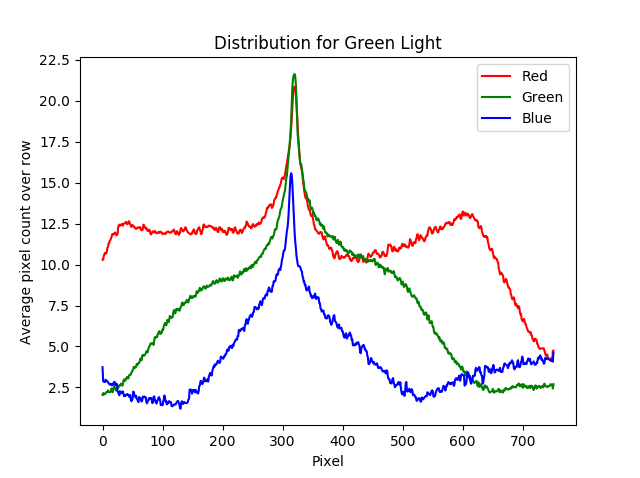
\includegraphics[scale=0.3]{greenDist.png}
\caption{The distribution of the average pixel count for the different colors when in the focal point of the green light. We see that while green has the largest average pixel count, red is close behind and for most of the image higher than green.}
\label{img:greenDist}
\end{figure}

The highest pixel counts for the given images are

\begin{table}[H]
\centering
\begin{tabular}{c | c | c | c}
Color in focus & Max Red & Max Green &Max Blue \\
\hline
Blue & $24$ & $137$ & $202$\\
Red & $255$ & $255$ & $255$\\
Green & $211$ & $255$ & $255$
\end{tabular}
\caption{The maximal pixel count for the different colors for the different focal points.}
\label{tab:colorMaxMin}
\end{table}




\subsection{Monochromatic Camera and Single Slit}
\label{sec:redMono}

\subsubsection{Bias and Dark Frame}
\label{sec:biasDark}

We started by looking at one bias and the dark frame for the maximum exposer.

\begin{figure}[H]
\centering

\includegraphics[scale=0.2]{df_max_exp.png}
\caption{Image of dark frame for maximum exposer.}
\label{img:df_max}
\end{figure}

\begin{figure}[H]
\centering

\includegraphics[scale=0.2]{bf1.png}
\caption{Image of a bias frame.}
\label{img:bf1}
\end{figure}

As we can see there are more or less the same. Lets look at some data about them:

\begin{table}[H]
\centering
\begin{tabular}{c|c|c}
 & Bias & Dark Frame \\
 \hline
 Max & 15 & 75 \\
 Min &6 & 4\\
 Max Location & $(439, 427)$ & $(214, 478)$\\
 Min Location & $(35, 528)$ & $(441, 84)$
\end{tabular}
\caption{Data about the bias and dark frame.}
\label{tab:biasDark}
\end{table}

The distribution of pixel values for the two are given as

\begin{figure}[H]
\centering
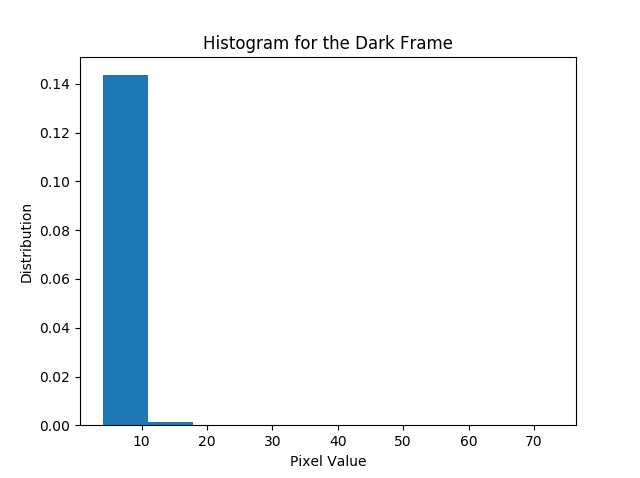
\includegraphics[scale=0.4]{histDark.png}
\caption{The distribution for the pixel values for the dark frame.}
\label{img:darkHist}
\end{figure}


\begin{figure}[H]
\centering
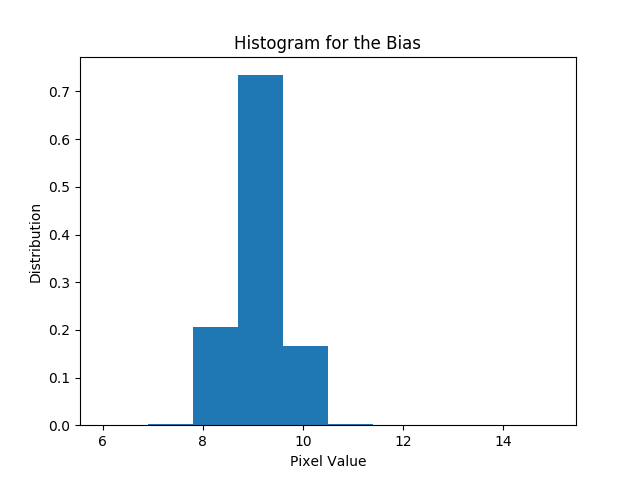
\includegraphics[scale=0.4]{histBias.png}
\caption{The distribution for the pixel values for the bias frame.}
\label{img:biasHist}
\end{figure}

\subsubsection{Bias, Flat Frame and Noise}
\label{sec:biasFlat}

For the analysis of the bias frames and two flat frames, the following data was obtained:

\begin{table}[H]
\centering
\begin{tabular}{c|c|c}
  & Bias & Flat Field \\
  \hline
Mean of sum & 17.99 & 141.80\\
Noise & 95.43 & 122.39
\end{tabular}
\caption{Data for the central regions of the bias frames, and the second and forth flat frames.}
\label{tab:biasFlat}
\end{table}


From the same bias and flat frames (flat frame 2 and 4) $g$ could be found as

\begin{equation}
g = 0.0210840557684  \text{ [electrons/ADU]}
\label{eq:gVal}
\end{equation}

And from a single bias frame the readout noise could be found

\begin{equation}
\text{R.O.N} = g\cdot\sigma_{bias} = 0.0210840557684\cdot0.592650538616 
\end{equation}
\begin{equation}
= 0.0124954770073 \approx 0.0125
\end{equation}


Using all of the 16 flat frames, we got the following result for the decrease in noise as a function of flat frames used:

\begin{figure}[H]
\centering
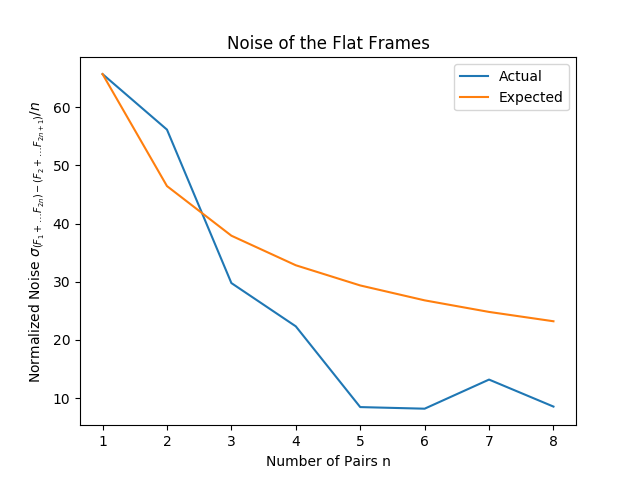
\includegraphics[scale=0.4]{noisePairs.png}
\caption{We can see as we use more and more pairs of flat frames, the noise decreases somewhere in order $1/\sqrt{n}$}
\label{img:noisePairs}
\end{figure}

\subsubsection{Pixel Size}
\label{sec:resPixSize}

The image taken for this calculation was as follows:

\begin{figure}[H]
\centering
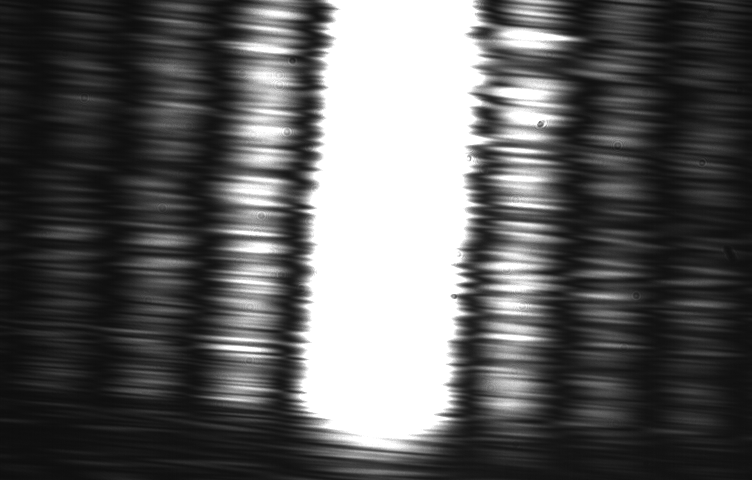
\includegraphics[scale=0.2]{3_1.png}
\caption{Image of the diffraction pattern with low exposer, used to find the pixel size.}
\label{img:rawPixSize}
\end{figure}

The middle slice of the image gave the following pixel values:

\begin{figure}[H]
\centering
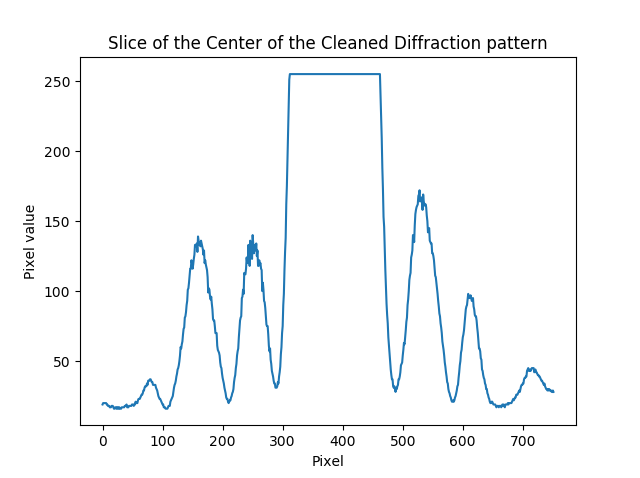
\includegraphics[scale=0.3]{slice.png}
\caption{A slice of the middle of the cleaned image of the diffraction pattern.}
\label{img:slice}
\end{figure}

If we look at the plot there are about 200 pixels from minimum to minimum, meaning that there are about $100$ pixels from the center to the first minimum. We discussed the uncertainty of the distance in pixels in sec. \ref{sec:uncSlit}. So adding that we get that

\begin{equation}
n_{pixels} = 100\pm 5
\end{equation}

We can then use \eqref{eq:pixelSize} to find the size of the pixels. We use that $m = 1$, $\lambda (641 \pm 12.3)$ nm \cite{laser}, $a = 100 \mu m$, and the measured distance from the slit to the CCD was $d = (8.5 \pm 0.2)$ cm:

\begin{equation}
c =  \frac{(641 \pm 12.3) \text{ nm} (8.5 \pm 0.2) \text{ cm}}{100\pm 5 \cdot100 \mu m} = (5.45 \pm 0.32)\text{ }\mu\text{m}
\end{equation}

So the size of one pixel of the CCD is $(5.45 \pm 0.32)\text{ }\mu\text{m}$.


\subsubsection{Cleaning the Scientific Image}

The raw of the diffraction pattern with slightly higher exposer was

\begin{figure}[H]
\centering
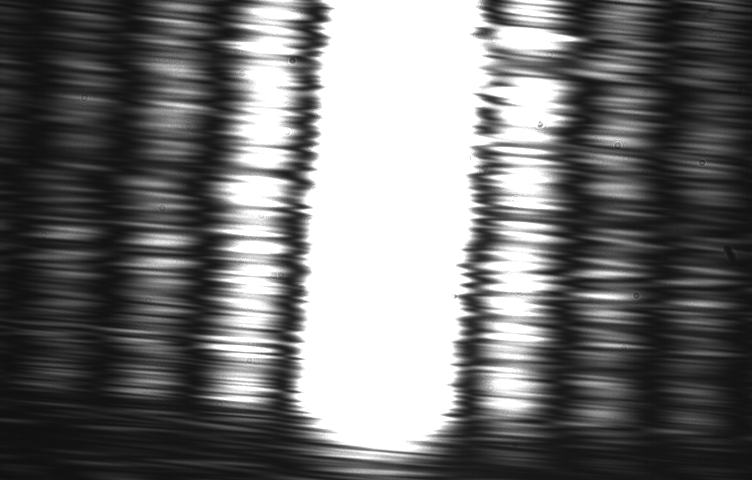
\includegraphics[scale=0.2]{3_2.png}
\caption{Image of the diffraction pattern, used to test the cleaning procedure.}
\label{img:rawClean}
\end{figure}

If we look close at the image one can see small circles. This is due to light diffracting of tiny dust particles somewhere on the instruments. This is some of the things we ideally want to remove with the flat fields.

After applying the cleaning procedure on the image we got the following result:

\begin{figure}[H]
\centering
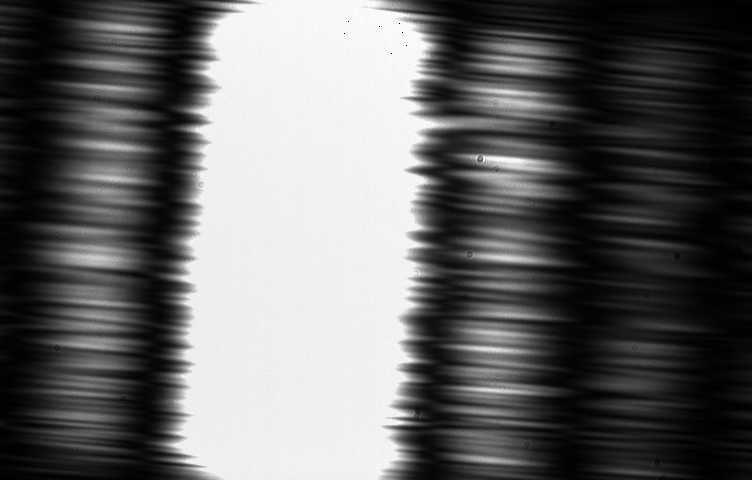
\includegraphics[scale=0.3]{corrected_image.png}
\caption{300x300 center part of the corrected image.}
\label{img:corr}
\end{figure}

\begin{figure}[H]
\centering
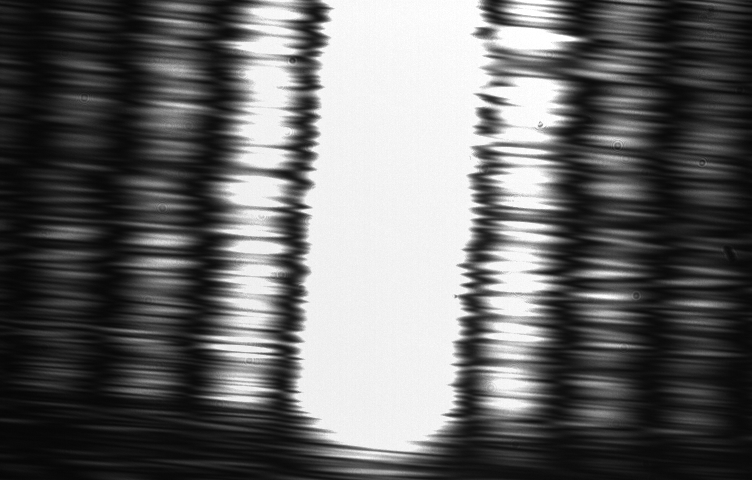
\includegraphics[scale=0.2]{corrected_image_fov.png}
\caption{The full field of view of the corrected image.}
\label{img:corrFOV}
\end{figure}






\section{Conclusions}
\label{sec:conclusions}

\subsection{Color Camera, White Light and Lens}
As we saw in sec. \ref{sec:resColor} we got different colors due to the chromatic aberrations of the lens. This effect made it so that we could move the CCD into the focal point of the different colors, letting us isolate the different colors. If we move the lens and camera so to remove the coma, a diffraction pattern can be observed. This is quite faint, but we can see a halo effect around the dot in the middle, which is due to the diffraction.

 If we then looked at the distribution of the mean pixel value of the different colors in the different focal points (\ref{img:blueDist}, \ref{img:greenDist} and \ref{img:redDist}) we saw that even though the images looked -- arguably -- monochromatic, all the colors contributed to some degree. This was most apparent for the green light, where both blue and red was abundant. We confirmed this by placing a red filter in front of the lamp, and while in the green focal point, the image lighted up red \ref{img:red_filter_green_focus}. Looking at table \ref{tab:colorMaxMin} we see that for the most part the color in focus has the largest maximum value. But it looks like we used a bit high exposer, making more that one color having the maximum pixel value (255) in some images. The strange part is that in the image of the green light we expected red to also have a high maximum pixel count, but as seen from the table blue has a higher maximum value than red. The reason for this remains unknown to the author, and requires more research.

\subsection{Monochromatic Camera and Single Slit}
\subsubsection{Bias and Dark Frame}
As we can see from fig. \ref{img:bf1} and \ref{img:df_max} the dark frame and bias is quite similar --mostly black. This is due to them both being made in the same way, with the dust cover on the camera. But if we look at the maximum and minimum values we see some difference. The minima of the two images are more or less the same, but the maxima are far apart. They are also not located at the same place, which should not be expected, since at least dark current is random in nature. This become more apparent from the distributions of pixel values, fig. \ref{img:biasHist} and \ref{img:darkHist}. Here we see that the dark frame has a larger share of higher pixel values. This may be due to the fact that the dark frame was recorded with the maximum exposer time, hence making the CCD more sensitive and recording higher pixel counts.

\subsubsection{Bias, Flat Frame and Noise}
From table \ref{tab:biasFlat} we see that both the bias and the flat frame has quite large mean and noise, but as expected those of the flat frames are higher -- since it is lit --. \\

The value for $g = 0.0211$ [electrons/ADU] seems quite small, since this means that we need about $1/50$ electrons to get signal. This also makes the readout noise small, R.O.N$=0.0125$ electrons. Other teams have calculated readout noise of close to $100$ \footnote{Can not cite this since it is from other students rapports}. The author are not sure why this is the case, but think it may have to do with the exposer of the camera: that changing the exposer drastically increases the readout noise\footnote{Not sure if it will increase with increasing or decreasing exposer.}. The conversion factor also varies drastically with different flat frames, and for frame 1 and 2 a negative factor is obtained. Why this is the case may also need further research.\\

If we look at fig. \ref{img:noisePairs} we see that we expected the noise to decrease with $1/\sqrt{n}$, but if we look at the actual noise it actually  decreases as $1/n$. The reason for this is unknown. It may simply be that we some noise in the noise, or that we have to few points to see that trend well. It may also be something wrong in the authors calculation of the noise. What ever the difference in the expected decrease and the calculated decrease, this is something that needs more research.

\subsubsection{Pixel Size}
We got a pixel size of $(5.45 \pm 0.32) \text{ }\mu$m, which is quite a good result, with a small uncertainty. But as discussed the number of pixels to the minimum may have been overestimated, and a larger uncertainty may be justified, or a better method of finding this distance needs to be found.\\

A better slit is also needed, to get more straight lines in the diffraction pattern. Better data on the wavelength of the laser will also give better results. Our wavelength was taken from only one source \cite{laser}, but in future calculations more samples of the wavelength should be used.

\subsubsection{Cleaning the Scientific Image}
\label{sec:disClean}
As seen in fig. \ref{img:rawClean} there are a lot of impurities in the picture. The most noticeable being the diffraction patterns made by dust on the instruments. Most of these impurities can be improved by the flat field\footnote{Dark current and bias being so small that cleaning these will have only a small difference.}. But if we look at the cleaned figures \ref{img:corr} and \ref{img:corrFOV} we see little difference. The diffraction patterns from the dust particles are still there. This is due to the ineffective way we made the flat frames:

Firstly: As discussed in under uncertainties, a piece of paper bends, making the flat frame less uniform. But the largest flaw was placing the paper right in front of the CCD. The dust observed in the images are most likely on the slit or objective. And since there were excluded from the flat frames, we have no way of correcting for these!

So to get a better, cleaner image we have to go back into the laboratory and get better flat frames with the objective and slit.\\

All in all the CCD has shown it self to be the future of image capturing -- especially if we manage to clean it correctly with the bias, dark and flat frames -- both due to it efficiency, but also due to its cheap price and ease of operation.


\bibliography{ref}



\begin{widetext}
\newpage
\section{Code}
\label{sec:code}
\textit{All the code have been tested on window 10, 64 bit, Python 3.5.2. The author can not guaranty that it will work on other computers and operating systems.}
\lstinputlisting{image_processing.py}
\end{widetext}

\end{document}
